\chapter{Proposed method}
We define a cache interaction, at the time of a cache eviction, in terms of the number of hits the evicted block will get compared to the number of hits the incoming block will get. Using this notion, we categorize the interactions as positive, negative and neutral interactions. For example, a cache block with 0 hits evicted by a cache block with 2 hits is identified as a positive interaction. The intuition behind this is, a useful cache block that will get 2 hits evicting a useless cache block that will not get any future hit is a desired situation with respect to the cache. The useless cache block would have consumed valuable cache space in case it was not evicted and still be resident in the cache. Similarly a useful cache block evicted by a useless cache block would consume valuable cache space as well as convert at least one hit to a miss for the useful cache block. We identify such an interaction as a negative interaction.
\\
As mentioned before, we are concerned about how cache management techniques and cache prefetchers interact with each other. So to capture this, we only take into account interactions where one of the blocks,i.e., either the incoming or the evicted block is a prefetched block. To be specific, we are only concerned about the following interactions:
 \begin{itemize}
        \item C evicts P
        \item P evicts P
        \item P evicts C
\end{itemize}
where P denotes a prefetched block which has not yet been demanded by the core and C denotes a cache block which has been brought in response to a demand request into the cache. 
\\
We argue that these interactions provide a good estimate of the actual interaction between cache management techniques and cache prefetchers for two reasons, (1) the category of an interaction depends on the decision taken by the cache prefetcher as we consider interactions with at-least one prefetched block and (2) the category of an interaction also depends on the decisions made by the cache managements technique it is the one taking all the eviction decisions. We are not concerned about the case \textbf{C evicts C} as it does not include prefetches and hence does not contribute to the overall interaction between cache management techniques and cache prefetchers. We will be looking into each of these scenarios in detail to characterize the interactions between prefetcher and cache replacement policies. 
\\\textbf{P evicts C}
\begin{enumerate}
    \item P evicts a dead C, where P gets a hit later. A dead block is nothing but a useless block. This can be characterized as a positive interaction as a useless C block is replaced by a useful P block.
    \item P evicts a non-dead C, where P gets a hit later. As C is non-dead it will be refilled into the cache at a later point of time. If C evicts the aforementioned P before it is used, then the whole interaction will be negative. On the other hand if C evicts the aforementioned P after P is used, then the whole interaction is neutral.
    \item P evicts a non-dead C, where P does not get a hit later. This can be characterized as a negative interaction as a useful block is replaced by a useless block.
    \item P evicts a dead C, where P does not a get a hit later. This interaction is neutral.
\end{enumerate}
\\
\textbf{C evicts P}
\begin{enumerate}
    \item A dead C evicts P, where P gets a hit later. This can be characterized as a negative interaction as a useless C block replaces a a useful P block.
    \item A dead C evicts P, where P does not get a hit later. This interaction is neutral.
    \item A non-dead C evicts P, where P gets a hit later. This can be characterized as a neutral interaction.
    \item A non-dead C evicts P, where P does not get a hit later. This can be characterized as a positive interaction as a useful C block replaces a a useless P block.
\end{enumerate}
\\
\textbf{P\textsubscript{1} evicts P\textsubscript{2}}
\\\\We assume P\textsubscript{1} as the prefetch block that is filled into the cache and P\textsubscript{2} as the prefetch block that is evicted from the cache.
\begin{enumerate}
    \item P\textsubscript{1} gets a hit later and P\textsubscript{2} does not get a hit later. This interaction is positive.
    \item P\textsubscript{1} gets a hit later and P\textsubscript{2} also gets a hit later. This interaction is neutral.
    \item P\textsubscript{1} does not get a hit later and P\textsubscript{2} also does not get a hit later. This interaction is also neutral.
    \item P\textsubscript{1} does not get a hit later and P\textsubscript{2} gets a hit later. This interaction is negative.
    
\end{enumerate}

In the next section we propose two techniques to implement the functionality of categorizing interactions into the different classes as discussed. As mentioned earlier, we need knowledge about future hits of blocks to classify each interaction as positive, negative or neutral. We first used a predictor based approach to estimate if a block would get a future hit or not and based on the prediction, categorized an interaction. But this approach is coarse grained as depends on heuristics to predict the future and in most workloads with varying memory access pattern, the predictions turn out to be incorrect. So we propose another method which tracks the future accesses of cache blocks associated with an interaction. This method gives near perfect estimation of interactions as it uses knowledge of the future cache access.
\section{Predictor based}
Two cache blocks are associated with a single interaction, the one which is evicted and the one which is incoming. To correctly categorize an interaction we need to predict the future hits of the two cache blocks. For the one that is evicted, future hits mean the number hits it would have got if it would be still in the cache. And for the incoming cache block, naturally it is just the number of cache hits it gets. However, due to the limitations of the predictor method we can only predict if a block will get a future hit or not rather than the number of future hits. This results in some of the positive or negative interactions to be predicted as a neutral interaction.
\\
We use a global hysteresis based dead block predictor as it is simple to implement and dynamically adapts to the dynamic program behavior. We make use of 3-bit global hysteresis counter. The counter is incremented whenever a cache block is evicted from the LLC without receiving any hits, and decremented whenever a cache block receives a hit. At the time of prediction if the counter is saturated, the block is predicted to be a dead block. To categorize an interaction we use this global hysteresis counter to make the prediction at the time of an eviction.
\begin{figure}[h]
  \centering
    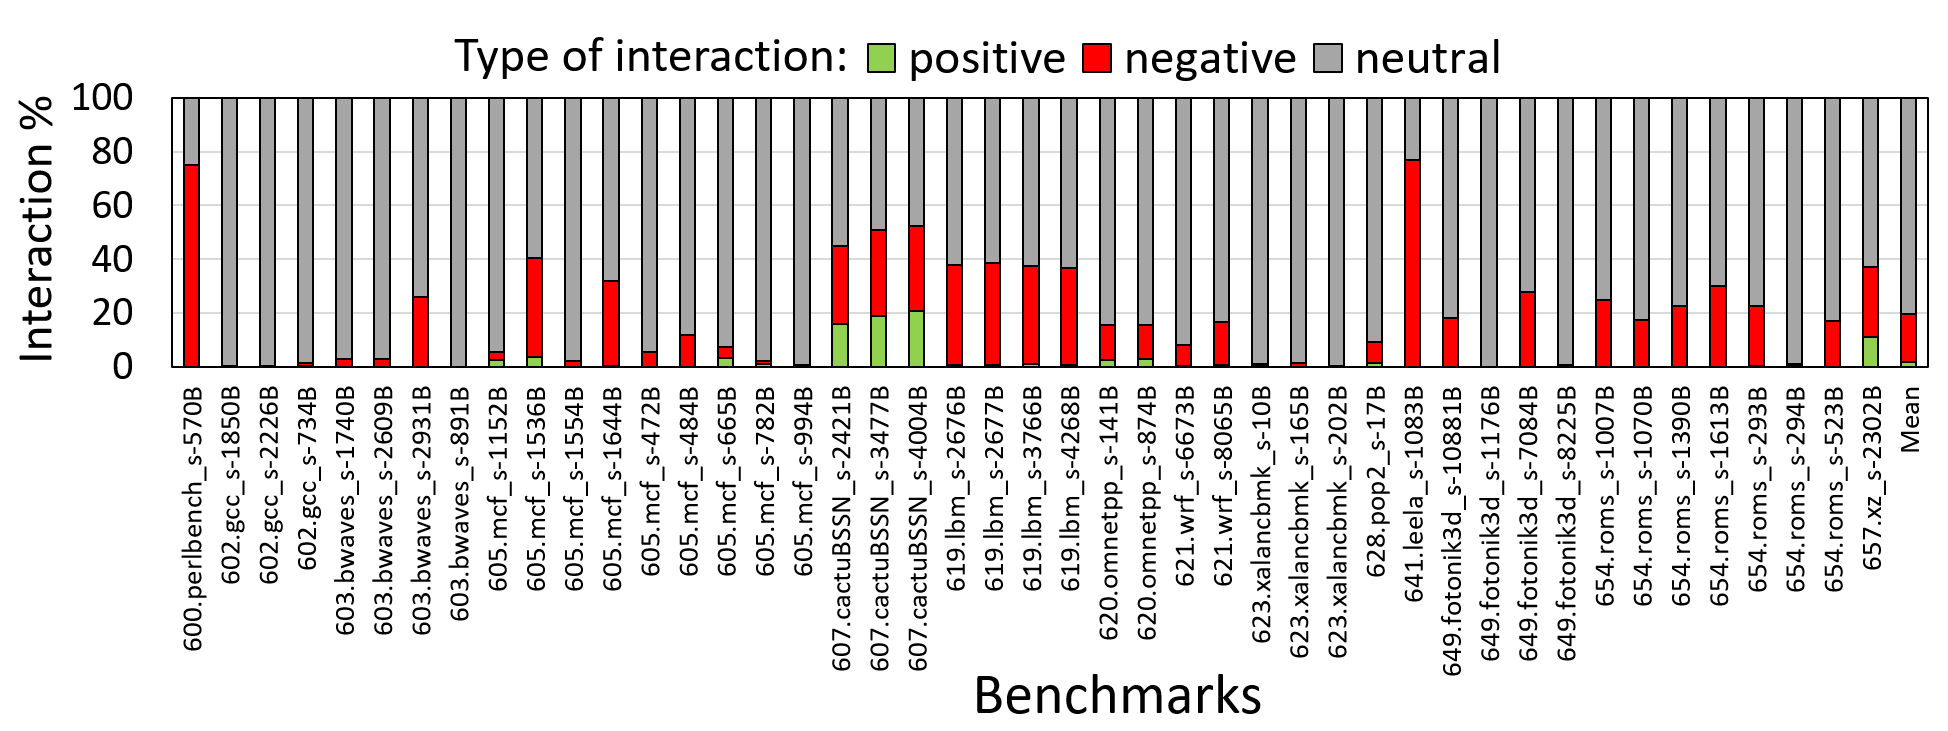
\includegraphics[width=1\textwidth]{lit/predictor_ipcp.png}
    \caption[Percentage of interactions for IPCP and Hawkeye]{Percentage of interactions for IPCP and Hawkeye using predictor method}
    \label{fig:pred_1} 
\end{figure}
\begin{figure}[h]
  \centering
    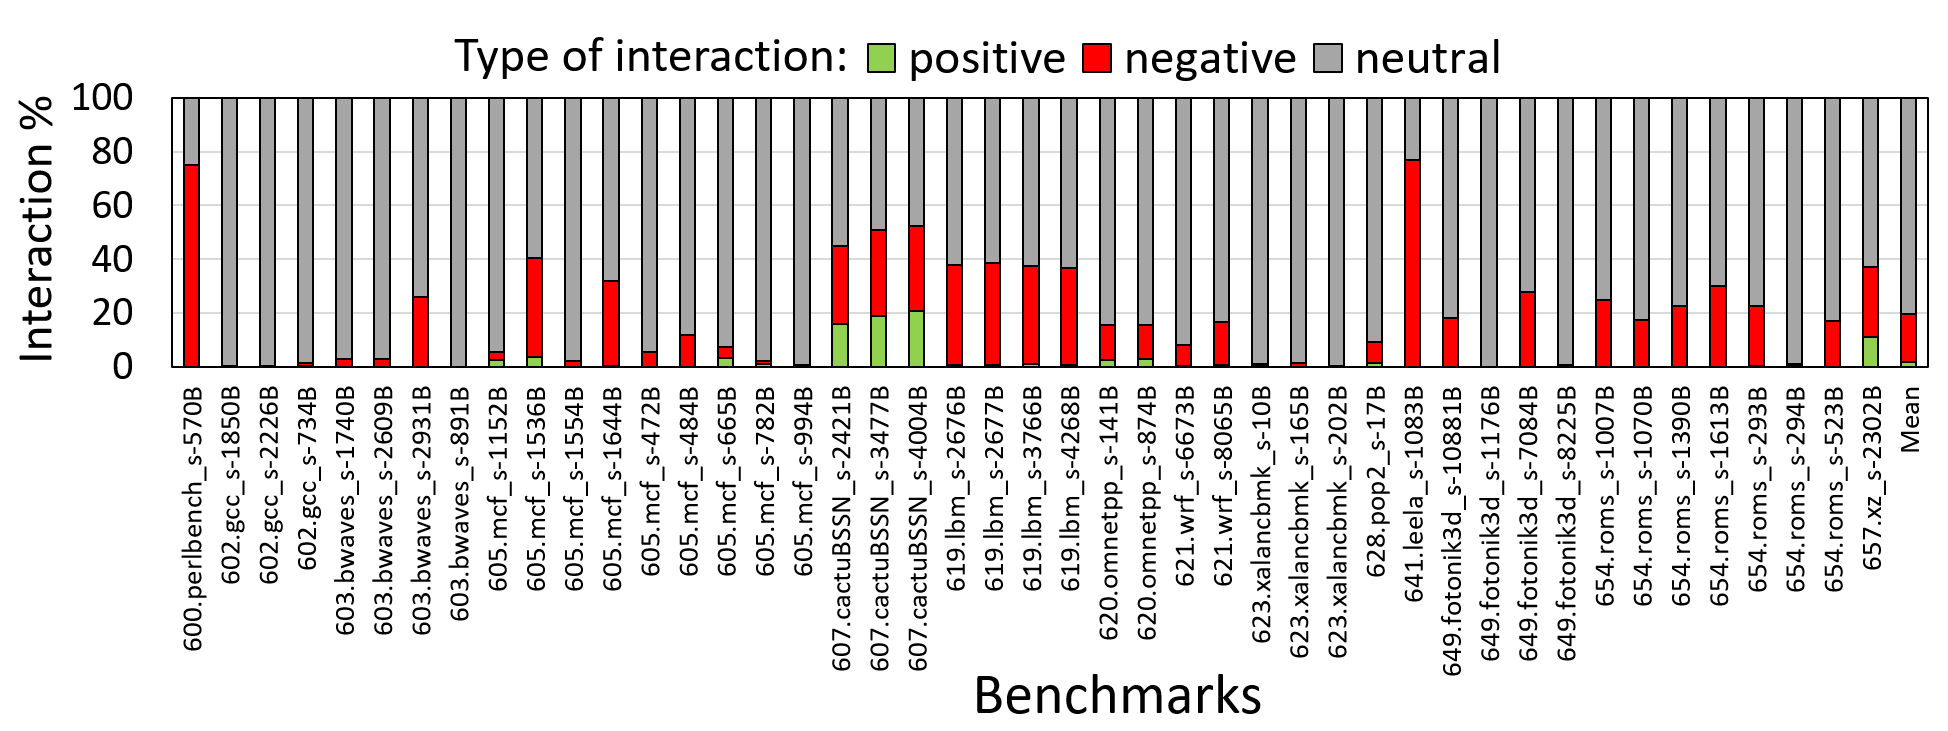
\includegraphics[width=1\textwidth]{lit/predictor_ipcp.png}
    \caption[Percentage of interactions for SPP and SHiP++]{Percentage of interactions for SPP and SHiP++ using predictor method}
    \label{fig:pred_2} 
\end{figure}

\section{Future access based}
In this approach we use a table to store all the interactions, i.e., the evictions entries as shown in figure \ref{fig:table_method}. Interactions are classified only until a certain epoch is reached, where epoch size is defined in terms of the number of cache evictions. For our experiments we set the epoch size to 2 times the cache size which is enough to track the future hits of the cache blocks involved in an interaction. We also store accesses to all cache blocks made within the epoch to track the future hits of cache blocks involved in an interaction. When an epoch is reached the table is parsed in a bottom-up fashion where each interaction is categorized using the hit count of respective cache blocks which is available from the cache access information stored in the table. 
\begin{figure}[h]
  \centering
    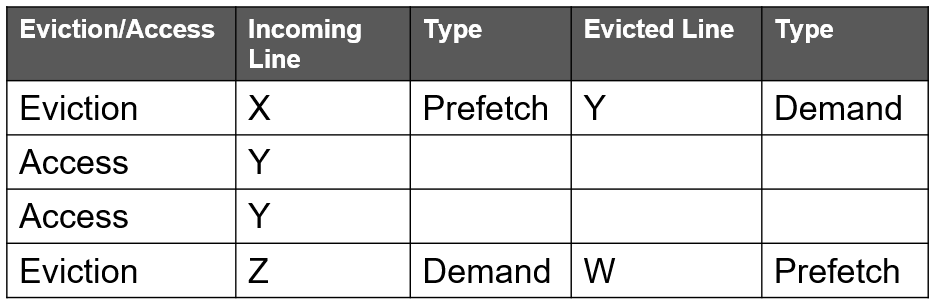
\includegraphics[width=1\textwidth]{lit/table_method.png}
    \caption[Table used for future access based method]{Table used for future access based method}
    \label{fig:table_method} 
\end{figure}
Unfortunately, the fact that this method requires knowledge about the future makes it an impractical approach. Although impractical, the data generated using this method is accurate and we use it to measure the ideal performance improvement for the case where we remove all the negative interactions. Although it is impossible to remove all the negative interactions in a practical system, the ideal performance improvement gives us a upper bound for achievable performance improvement. In the next section we will look into the details of the model used to measure the ideal performance improvement.

\begin{figure}[h]
  \centering
    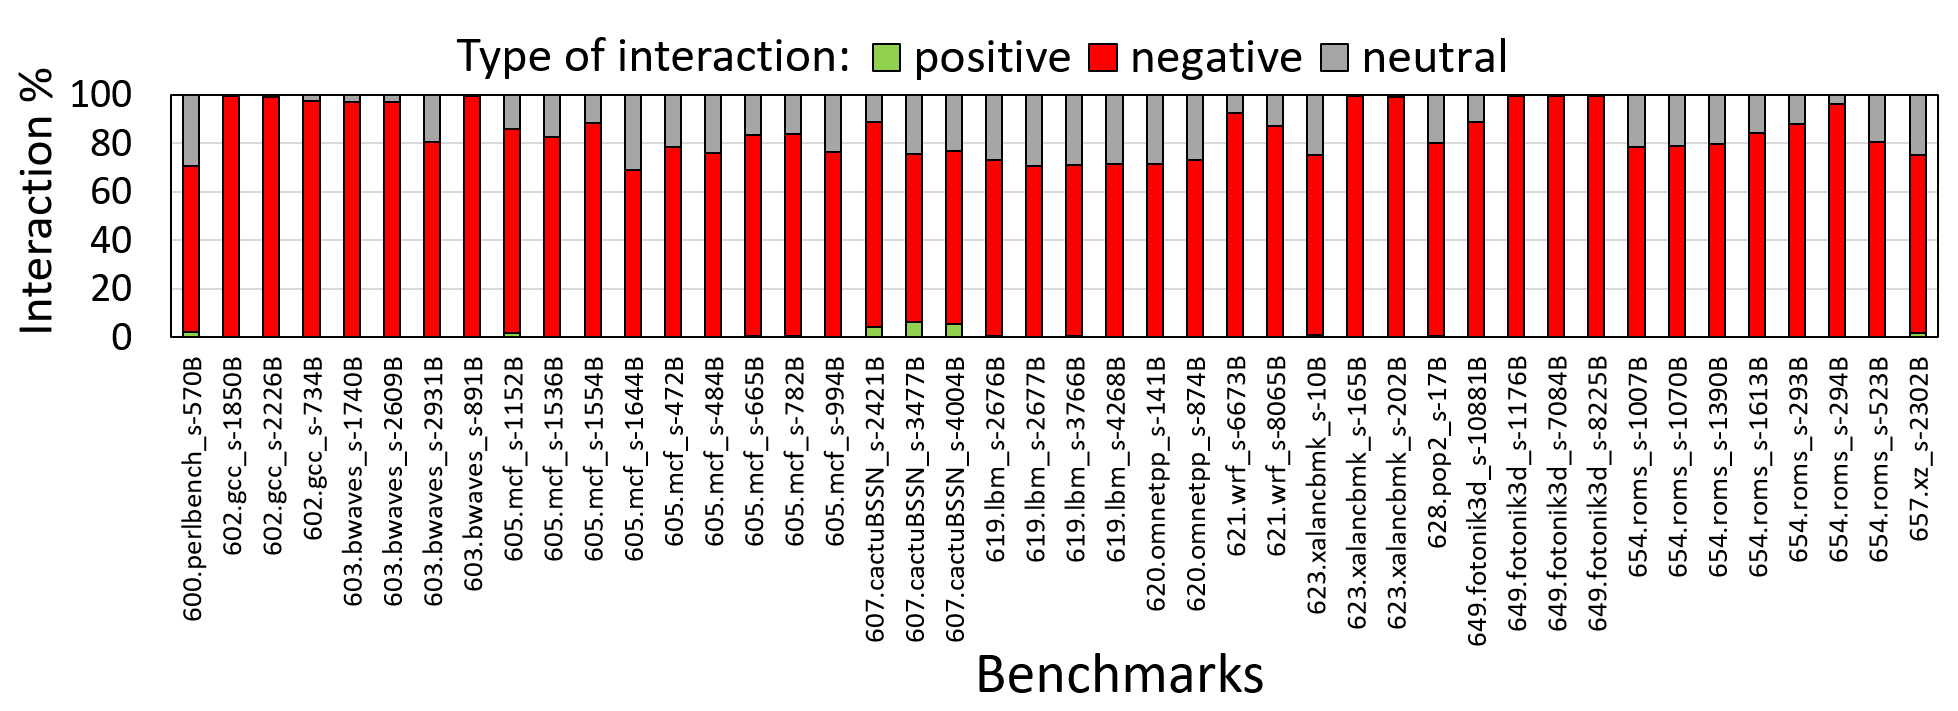
\includegraphics[width=1\textwidth]{lit/table_ipcp.png}
    \caption[Percentage of interactions for IPCP and Hawkeye using predictor method]{Percentage of interactions for IPCP and Hawkeye using future access based method}
    \label{fig:table_method} 
\end{figure}

\begin{figure}[h]
  \centering
    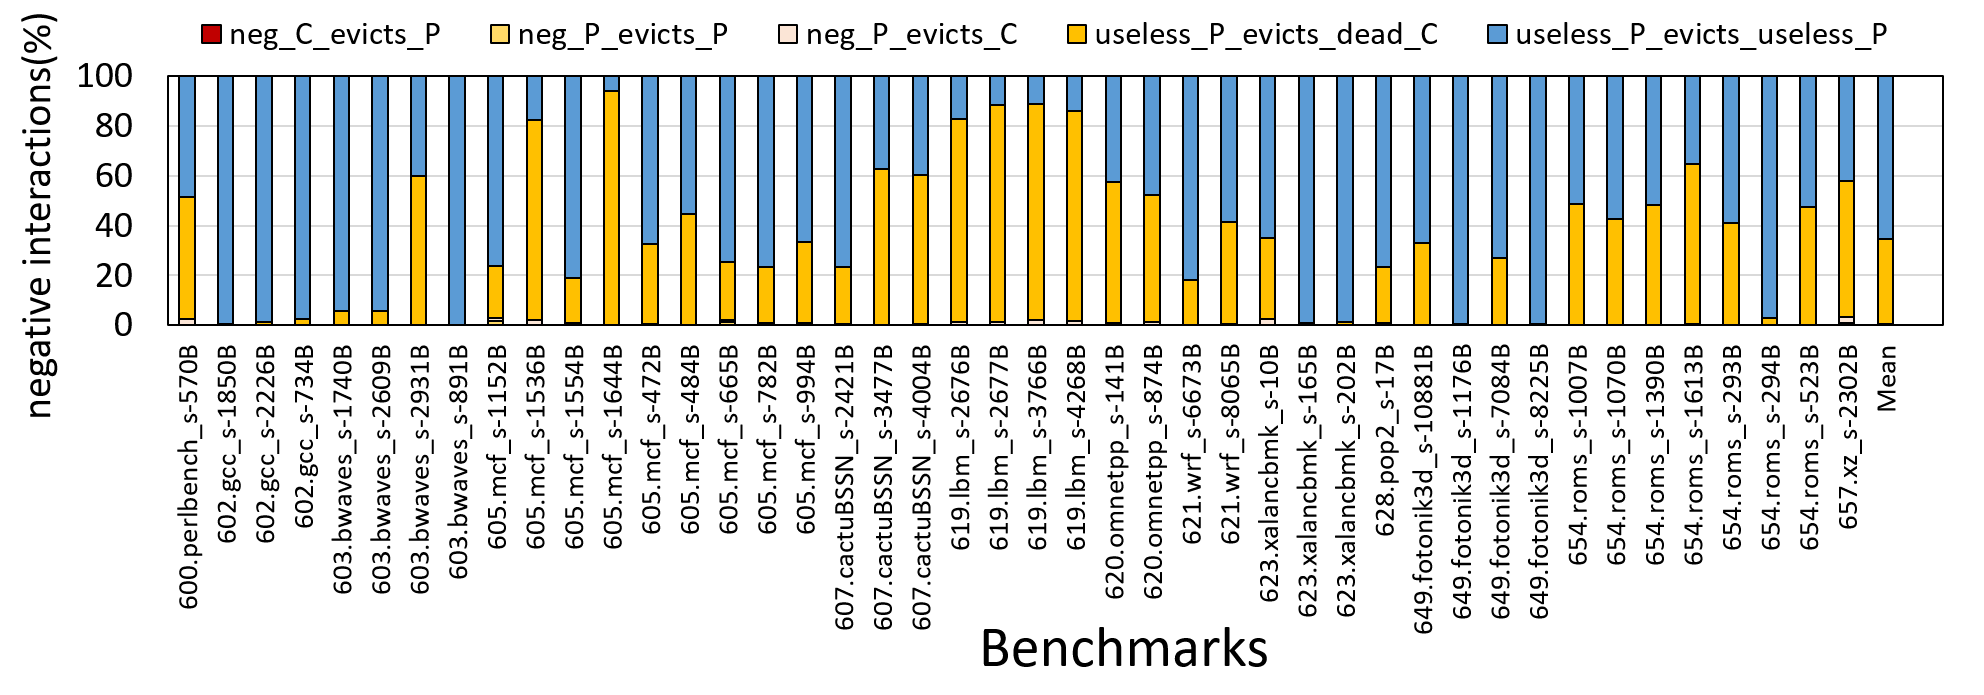
\includegraphics[width=1\textwidth]{lit/table_ipcp_neg.png}
    \caption[Breakdown of negative interactions for IPCP and Hawkeye using predictor method]{Breakdown of negative interactions for IPCP and Hawkeye using future access based method}
    \label{fig:table_method} 
\end{figure}

\section{Ideal performance improvement}
In this section we will measure the ideal performance improvement possible when we remove all negative interactions. We call it ideal as it is near to impossible to eliminate all the negative interactions in a real system. However, this will give an upper limit of the maximum performance improvement possible. We propose a mathematical model to find the performance improvement on eliminating negative interactions. From the perspective of LLC, the negative interaction hog the DRAM bandwidth, which introduce an additional latency on every DRAM access. Let the additional delay introduced by the negative interactions the negative interactions per DRAM access be $P$. Thus every load request from the CPU that goes to the DRAM suffers an additional latency of $P$. And the load requests that go to the DRAM are nothing but the loads that miss in the LLC. We define the additional latency per LLC Miss ($P$) as follows:
\begin{equation}
    P = avg. \ miss \  latency \ with \  \ prefetcher - avg. \  miss \ latency \ without \ prefetcher
\end{equation}
But in addition to this, we need to keep two additional things in mind. First, as we are dealing with an out-of-order processor, multiple load instructions can be waiting for a memory operation to complete in parallel. Secondly, with the support of Miss status holding registers(MSHR) multiple load instructions can miss at the LLC and wait for the miss to get resolved in parallel. So, considering there are multiple LLC misses from multiple instructions waiting in the MSHR, the additional penalty will amortized over all the loads active in the MSHR. We use the average MSHR occupancy as a proxy for the average number of loads active in the MSHR. Thus, we can define the additional latency per LLC miss ($P$) as:

\begin{equation}
    P = \frac{avg. \ miss \  latency \ with \  \ prefetcher - avg. \  miss \ latency \ without \ prefetcher}{avg. \ MSHR \ occupancy}
\end{equation}
Let $F$ be the fraction of LLC misses that suffers from this penalty, so we can define $F$ as:
\begin{equation}
    F = num \ of \ LLC \ misses \times fraction \ of \ negative \ interactions
\end{equation}
Using these quantities F and P we can easily find the improved metric instructions per clock cycle(IPC) as follows:
\begin{equation}
    IPC(no \ negative \ interaction) = \frac{number \ of \ instructions}{cpu \ cycles - F \times P}
\end{equation}

\section{Evaluation}
In this section we will be looking into the overall performance improvement for a fixed prefetcher with varying cache management techniques at the LLC. The baseline for all cases is a system with LRU cache management technique without any prefetching. Figure 2.6 and 2.7 shows the performance improvement for SPEC2017 benchmarks and figure 2.8 and 2.9 shows the performance improvement for GAP benchmarks.


\begin{figure}[h]
  \centering
    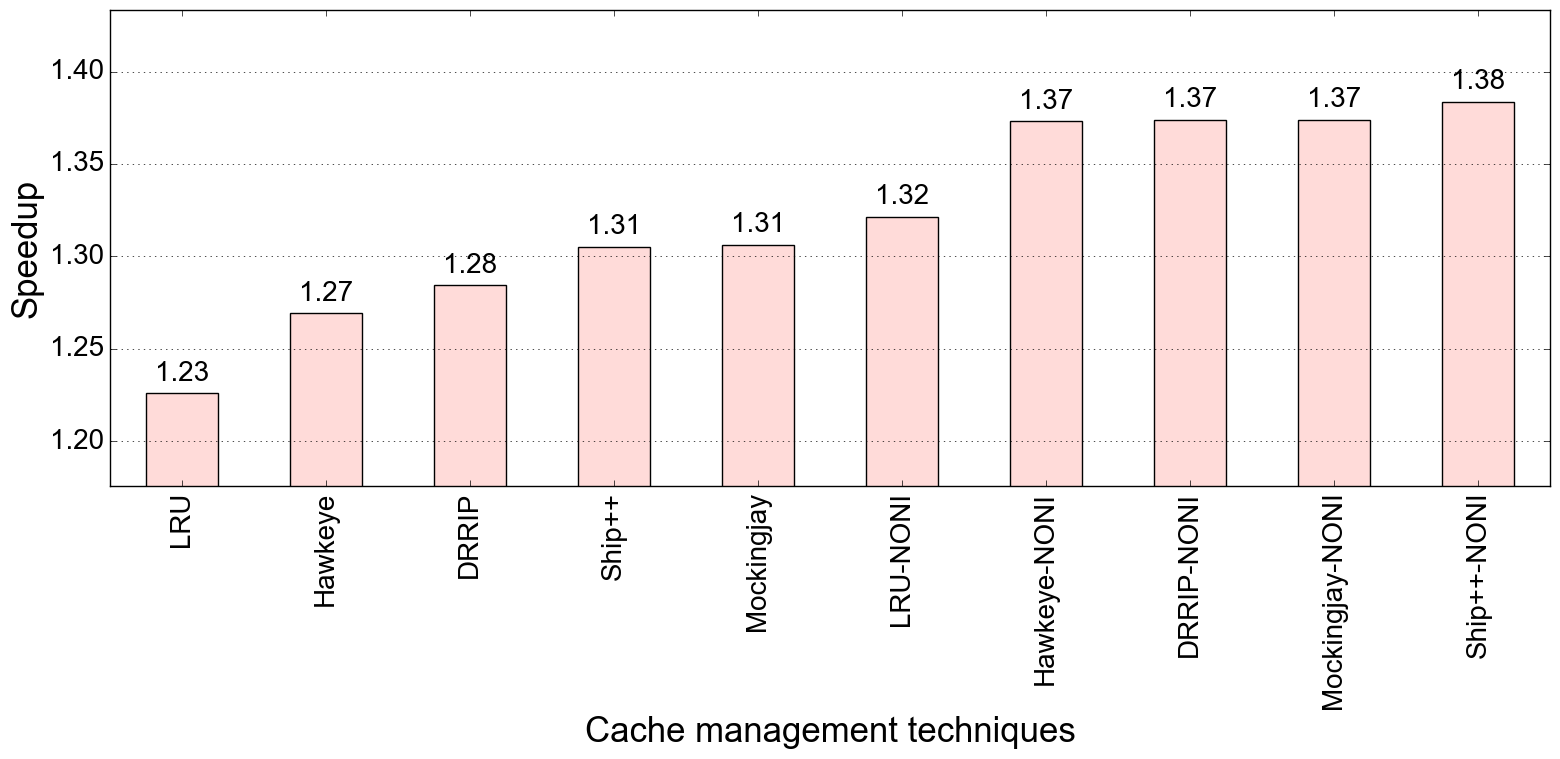
\includegraphics[width=1\textwidth]{lit/800_ipcp_geomean.png}
    \caption[Percentage of late prefetches of IPCP for low and high DRAM bandwidth on SPEC2017 benchmarks]{Performance improvement without negative interactions for IPCP prefetcher with varying management techniques on SPEC2017 Benchmarks}
    \label{fig:late} 
\end{figure}

\begin{figure}[h]
  \centering
    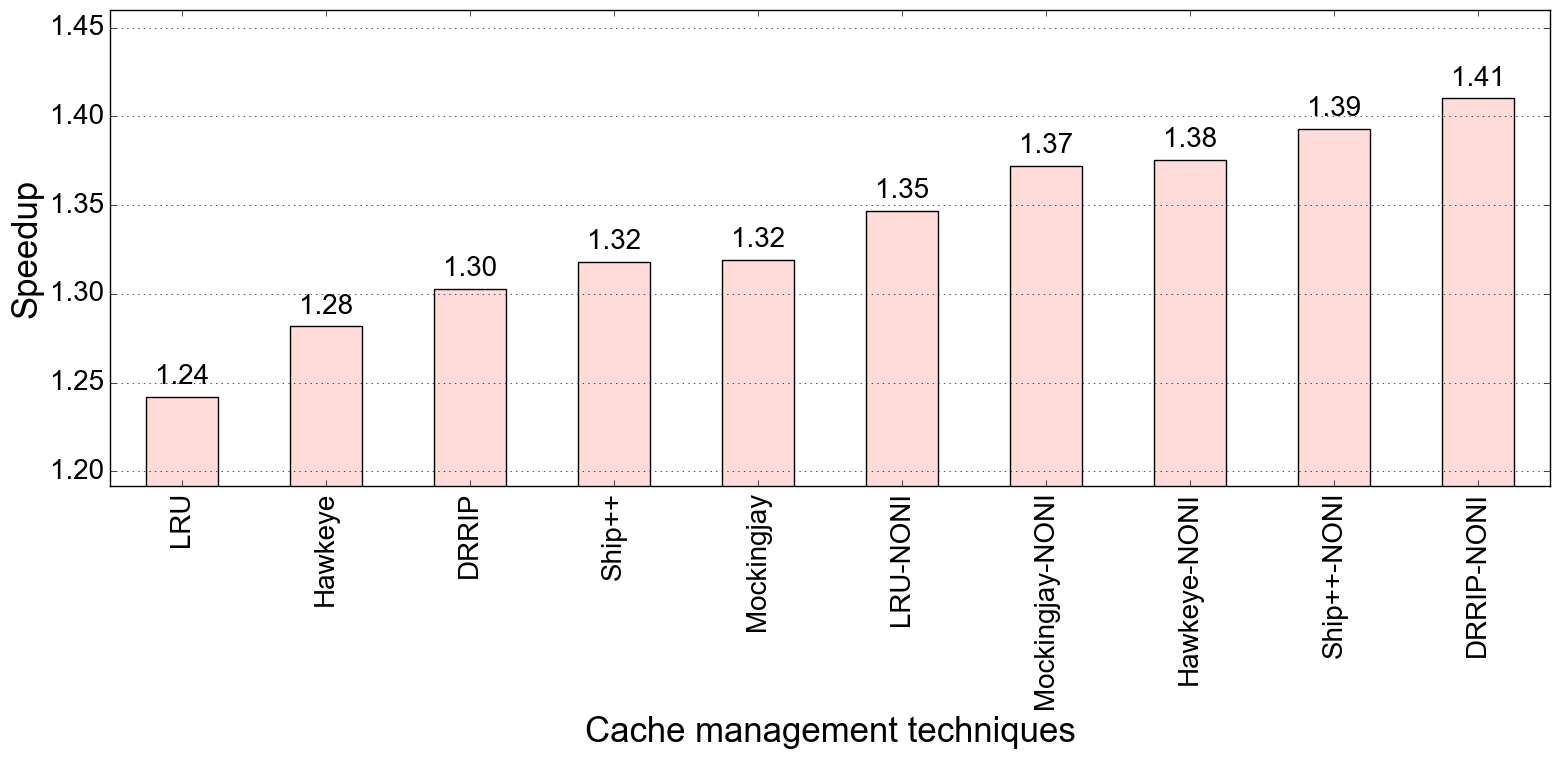
\includegraphics[width=1\textwidth]{lit/800_ipStrideNl_geomean.png}
    \caption[Percentage of late prefetches of IPCP for low and high DRAM bandwidth on SPEC2017 benchmarks]{Performance improvement without negative interactions for IP-stride and Next Line prefetcher with varying management techniques on SPEC2017 Benchmarks}
    \label{fig:late} 
\end{figure}

\begin{figure}[h]
  \centering
    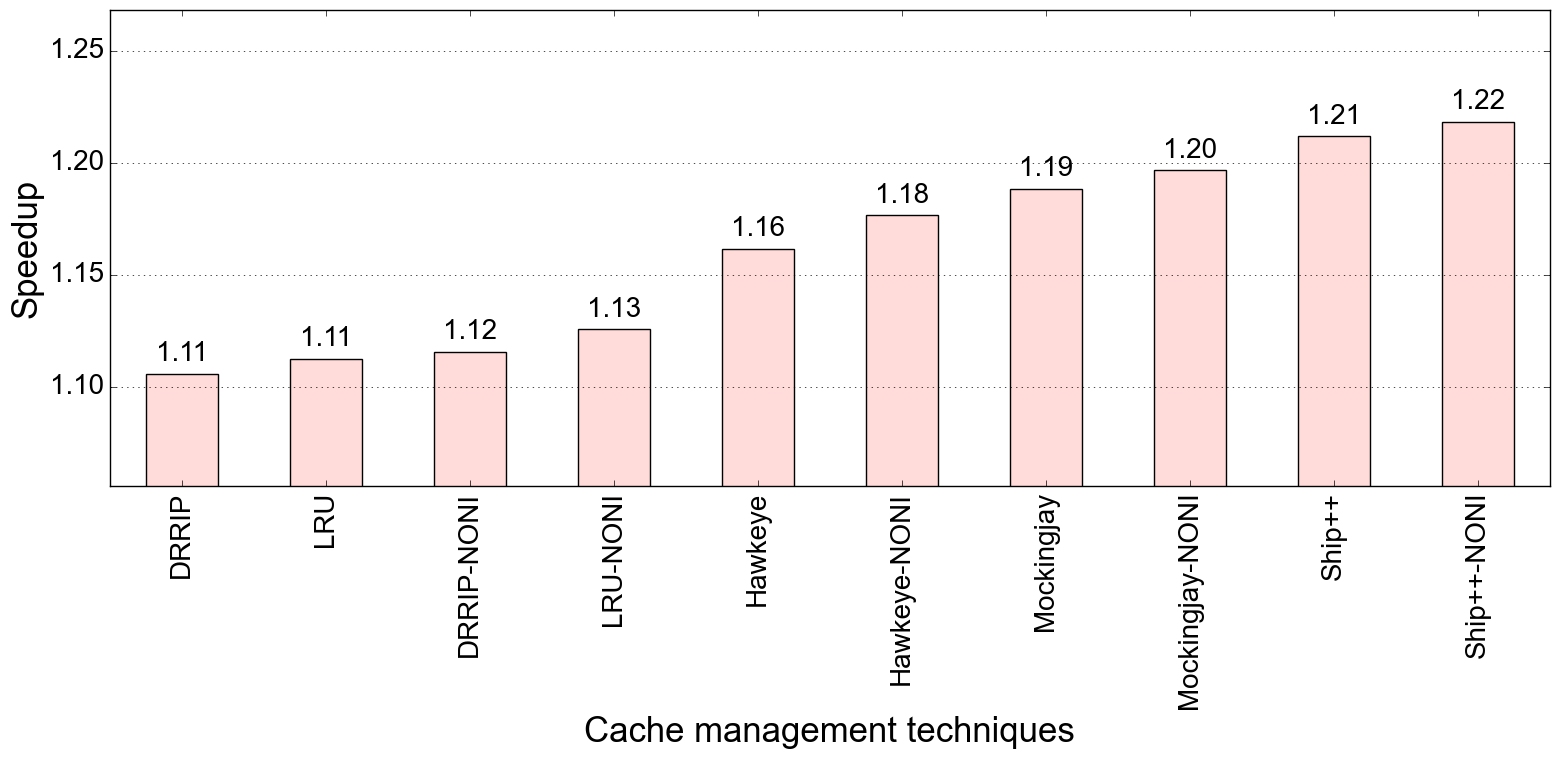
\includegraphics[width=1\textwidth]{lit/800_spp_geomean_gap.png}
    \caption[Percentage of late prefetches of IPCP for low and high DRAM bandwidth on SPEC2017 benchmarks]{Performance improvement without negative interactions for SPP prefetcher with varying management techniques on GAP Benchmarks}
    \label{fig:late} 
\end{figure}

\begin{figure}[h]
  \centering
    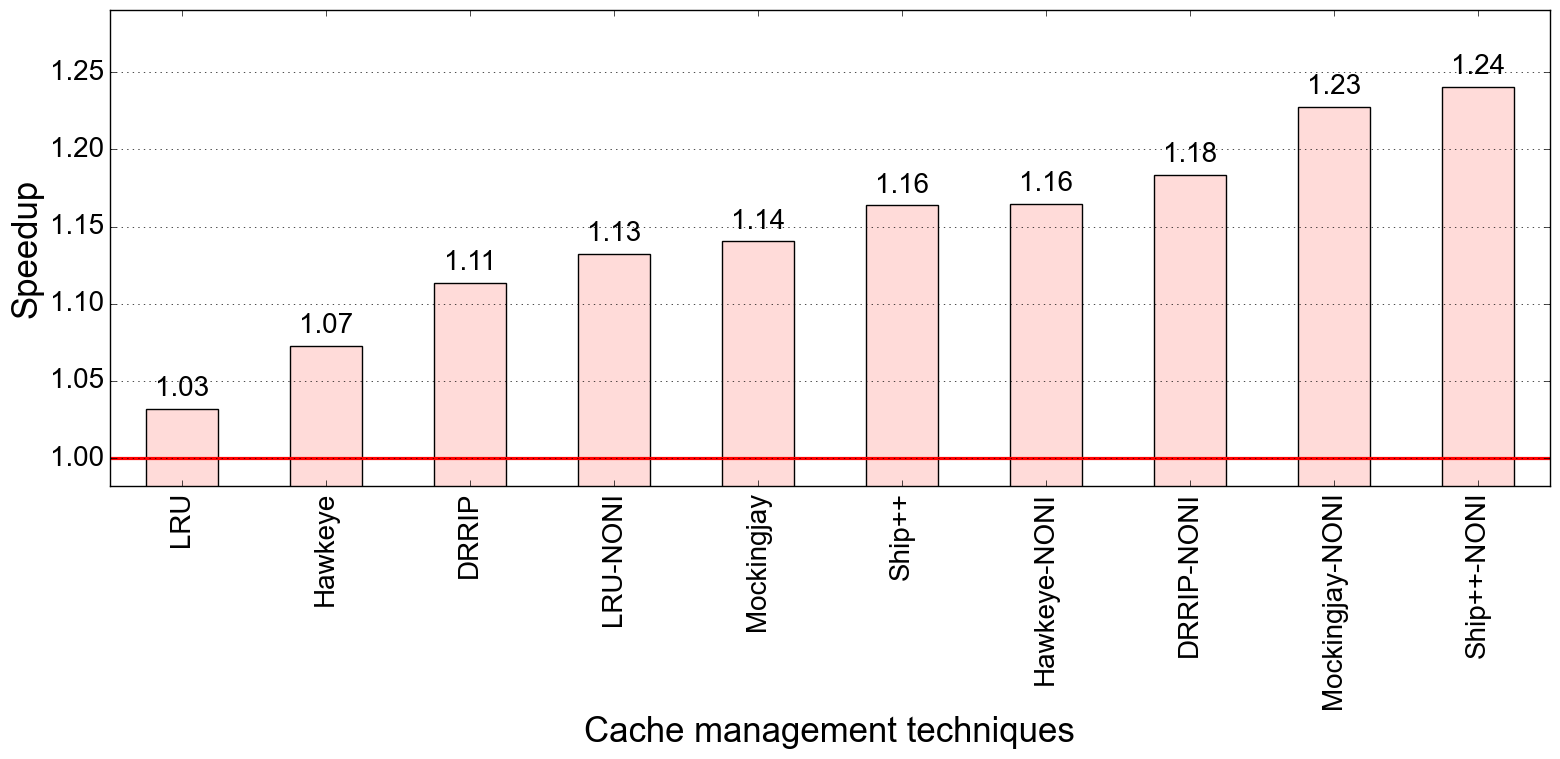
\includegraphics[width=1\textwidth]{lit/800_ipStrideNl_geomean_gap.png}
    \caption[Percentage of late prefetches of IPCP for low and high DRAM bandwidth on SPEC2017 benchmarks]{Performance improvement without negative interactions for IP-stride and Next Line prefetcher with varying management techniques on GAP Benchmarks}
    \label{fig:late} 
\end{figure}

%%% Local Variables: 
%%% mode: latex
%%% TeX-master: "../mainrep"
%%% End: 
